\documentclass[twocolumn]{article}
\usepackage{geometry}
\usepackage[pdftex]{graphicx}
\usepackage[utf8]{inputenc}
\usepackage{algorithmic}
\usepackage{algorithm}
\usepackage{titlesec}

\titleformat{\section}{\large\bfseries}{\thesection}{1em}{}

\title{Contrast Enhanced Adaptive Luminance Tone Mapping for High Dynamic Range Image Visualization}
\author{Richard Monette}

\begin{document}

\maketitle

\section{Abstract}

In this paper, we present key enhancements to the tone mapping operator originally proposed by Duan et al.\cite{duan05} Specifically, by utilizing a superior histogram equalization technique we eliminate the need for a contrast user parameter and ensure optimal, brightness preserving contrast is achieved automatically. Additionally, a human visual system exploiting local contrast enhancement sub-operator is presented which improves image readability without distorting overall luminance levels.

\section{Introduction}

The ongoing proliferation of image capture hardware and physically based image synthesis software has created an increasing requirement for effective algorithms to map newly created high dynamic range image content for display on existing low dynamic range display hardware. This mapping process is handled by so-called tone mapping operators. Fundamentally, a tone mapping operator must perform two operations in order to perform this mappingl:

\begin{itemize}
\item Compress the high dynamic range luminances to the displayable range
\item Preserve (or recover) the luminace contrast information from the original image
\end{itemize}

Building on the research conducted by Duan et al.\cite{duan05}, our operator uses an adaptive luminance mapping followed by global and then local contrast enhancment stage. The adaptive luminance mapping compresses the image luminance levels into the displayable range. Then the specifically selected global and local contrast enhancements ensure final image quality and readability through optimal use of the displayable range. First, we present the Brightness Preserving Bi-Histogram Equalization algorithm which is the basis for the Minimum Mean Brightness Error Bi-Histogram Equalization algorithm which we use in our tone mapping operator. Then we explain how the local contrast is enhanced using an unsharp masking operation.
Finally, we present our results and comparision to existing tone mapping operators as well as a brief discussion of the performance characteristics of our operator. 

\section{Adaptive Luminance Mapping}

The luminance of the high dynamic range image $I$ is compressed to the displayable range $D$ using the following compression formula originally presented by Duan et al.\cite{duan05}

\begin{equation}
\triangle_D = (D_{max}-D_{min})
\end{equation}

\begin{equation}
D(I) = \triangle_D  * \frac{log(I) - log(I_{min})}{log(I_{max}) - log(I_{min})} + D_{min}
\end{equation}

where $I_{min}$ and $I_{max}$ are the minimum and maximum luminace of the real scene and $D_{min}$ and $D_{max}$ are the minimum and maximum luminances the visualization device is capable of reproducing. In the original formulation a brightness scale factor is included however when a brightness preserving contrast enhancement is used the need for this parameter is eliminated. It is worth noting that any suitable luminance mapping formula which performs an equivalent compression could be interchanged. Examples of equivalent compression approaches can be found in the tone mapping operator research of Drago\cite{drago03} and Reinhard\cite{reinhard02}.

\section{Global Contrast Enhancement}

After the adaptive luminance mapping has been completed, the resulting image will have reduced contrast and detail as a result of the compression. This is because the luminance mapping is done purely on the basis of luminance without taking into account the luminance distribution characteristics of the overall image. Thus, the mapped image may be under or over utilizing certain luminace values. In order to ensure that the full range range luminance values is optimally utilized a traditional histogram equalization operation could be performed. However, one of the characteristics of naive historgram equaliztion is that the overall brightness of the image signal is modified. This results in incorrectly dark results and/or undesirable artifacts. In order to control this darkening, Duan et al. found it neccessary to utilize a 'linear equal' mapping. The 'linear equal' mapping requires the user to adjust a blending variable which controls the linear blending of the source image signal with that of the naive histogram equalized signal. We note that Ward accounts for various different human visual system factors but also does not directly address the specific limitations of the historgram equalization technique itself.\cite{ward97} However, as we demonstrate, using the more sophisiticated minimum mean brightness error bi-histogram equalization algorithm the overall brightness is preserved. By preserving overall brightness,  the requirement for a contrast adjustment parameter is eliminated. Eliminating this parameter allows for better images to be produced automatically.

\subsection{Brightness Preserving Bi-Histogram Equalization (BBHE)}

The BBHE algorithm bi-partitions the image around the mean luminance and performs two seperate histogram equalizations. These two sub-images are then recombined to produce the final result. By partitioning the image and performing two seperate histogram equalization operations, it is possible to better preserve the overall brightness in comparision to naive histogram equalization where the output mean is always the middle grey level.\cite{kim96}

\begin{figure}[h!]
	\centering
	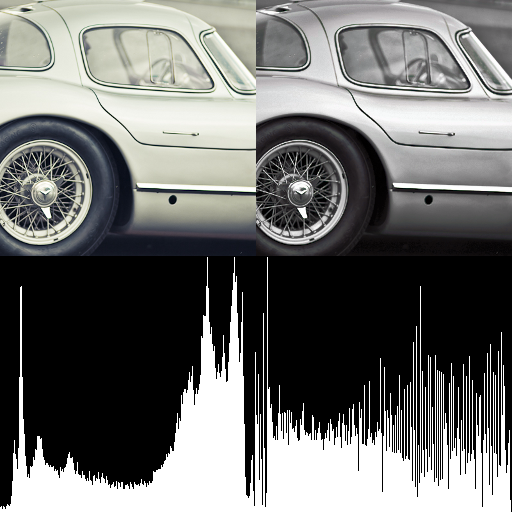
\includegraphics[scale=0.5]{regular_histogram_car}
	\caption{Example of naive histogram equalization}
\end{figure}

\begin{figure}[h!]
	\centering
	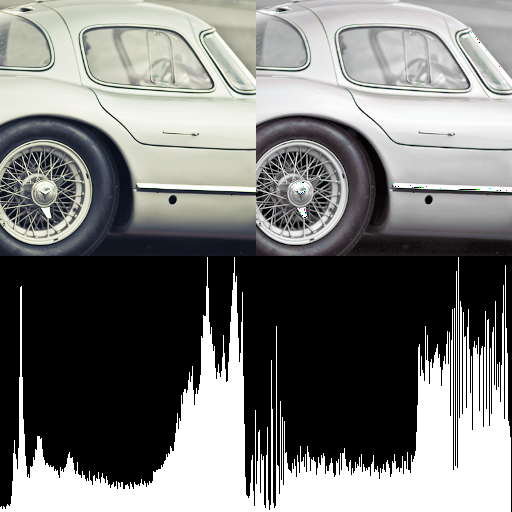
\includegraphics[scale=0.5]{regular_bright_histogram_car}
	\caption{Example of Brightness Preserving Bi-Histogram Equalization}
\end{figure}

\subsection{Minimum Mean Brightness Error Bi-Histogram Equalization in Contrast Enhancement (MMBEBHE)}

Although the BBHE algorithm improves the accuracy of the output brightness of an equalized image, further examination reveals that the mean is not the optimal parition position. An optimal partition can be found by utilizing the MMBEBHE algorithm.\cite{wang05} The MMBEBHE algorithm determines the optimal partition by examining the Absolute Mean Brightness Error (AMBE) of each potential partition. Once the AMBE has been calculated for each potential partition, the lowest error postion is used.\cite{chen03} The AMBE is defined as the absolute difference between the input and output mean. 

The MMBEBHE algorithm uses the following procedure:

\begin{itemize}
\item Calculate the AMBE for each potential partition
\item Select that partition which yields the lowest error
\item Partition on this position
\item Perform the bi-histogram equalization (as in BBHE)
\end{itemize}

\section{Local Contrast Enhancement}

By using the MMBEBHE algorithm we ensure that the full range of displayable luminances is optimally utilized. A further increase in output image quality can be achieved by enhancing the local contrast of image details and transitions in the luminance signal.

\subsection{The Cornsweet Illusion}

The Cornsweet illusion is an optical phenomena that affects the human visual system in which two regions, that are in reality of equal brightness, appear to be of different brightness due to a gradient at the edge along which they meet.\cite{purves99}

\begin{figure}[h!]
	\centering
	
\includegraphics[scale=0.375]{cornsweet}
	\caption{Actual versus perceived signal\cite{wiki_corn}}
\end{figure}

This phenomena can be exploited to great advantage in the tone mapping process as it allows for adding apparent contrast while not requiring modification of overall luminances.

\subsection{Unsharp Masking}

Unsharp masking is an image processing technique which enhances acutance on image details. The 'unsharp mask' is created by subtracting a Gaussian blurred version of the source image from the original image. This mask is then used to blend between the original and a globally contrased enhanced image. To produce our globally contrast enhanced image we use a Laplacian sharpening kernel. 

\begin{figure}[h!]
	\centering
\[  \begin{array}{ccc}
-1 & -1 & -1 \\
-1 &  8 & -1 \\
-1 & -1 & -1 \end{array} \] 
\caption{Laplacian sharpening kernel}
\end{figure}

In our experiments we used a three pixel radius in our Gaussian blur. The result of using the unsharp masking procedure is enhanced local contrast created by edge gradients which induce the Cornsweet phemonema in the viewer.

\begin{figure}[h!]
	\centering
	
\includegraphics[scale=1.0]{unsharpmask3}
	
\includegraphics[scale=1.0]{unsharpmask1}
	\caption{Example of original and then sharpened image segment\cite{unsharp}}
\end{figure}

\begin{figure}[h!]
	\centering
	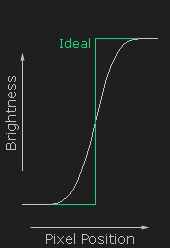
\includegraphics[scale=0.5]{unsharpmask2}
	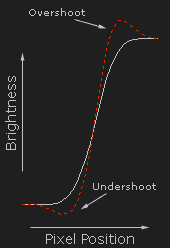
\includegraphics[scale=0.5]{unsharpmask}
	\caption{Left: Normal signal showing with theoretical ideal overlayed Right: Unsharp mask signal overlayed\cite{unsharp}}
\end{figure}

An additional advantage is conferred by conducting the local contrast enhancement on the luminance signal, as it ensures that color artifacts that sometimes are a result of unsharp masking color images will not occur.

\begin{figure}[h!]
	\centering
	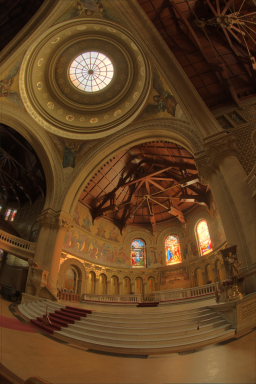
\includegraphics[scale=0.5]{memorial_no_contrast}
	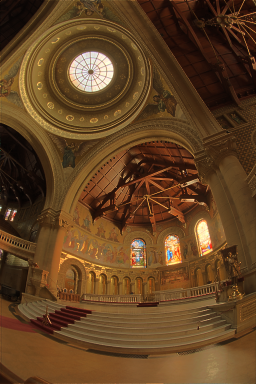
\includegraphics[scale=0.5]{memorial_contrast}
	\caption{Memorial scene tone mapped without (left) and with (right)  local contrast enhancement}
\end{figure}

\section{Results}

For our testing, we implemented the original Duan et al. algorithm and then compared our output with the reference program provided. Having established that our implementation created identical output we then applied our upgraded contrast enhancements operations.

\begin{figure}[h!]
	\centering
	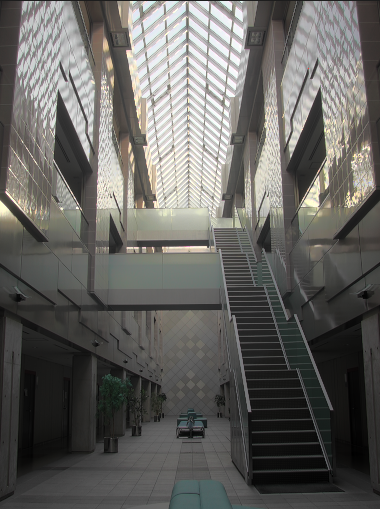
\includegraphics[scale=0.5]{atrium_morning}
	\caption{Atrium scene in morning.}
\end{figure}

\begin{figure}[h!]
	\centering
	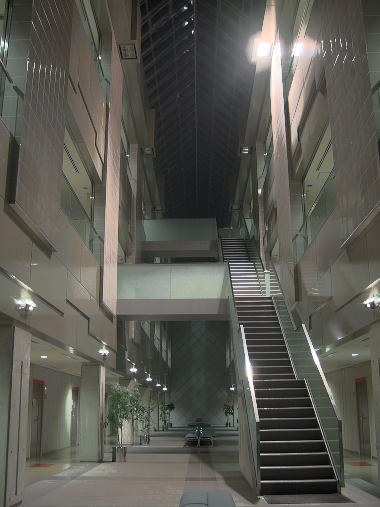
\includegraphics[scale=0.5]{atrium_night}
	\caption{Atrium scene in night. Note that no parameters required adjustment for these images because of the brightness preserving histogram equalization.}
\end{figure}

\begin{figure}[h!]
	\centering
	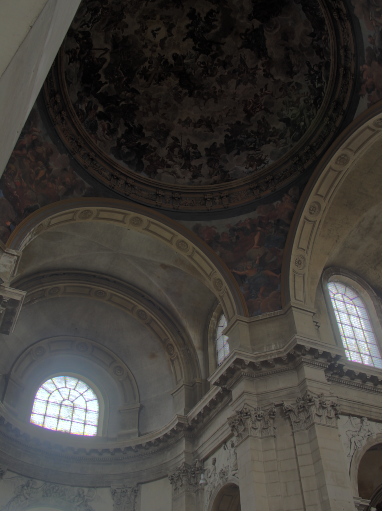
\includegraphics[scale=0.5]{cathedral}
	\caption{Cathedral scene mapped with our operator}
\end{figure}

\begin{figure}[h!]
	\centering
	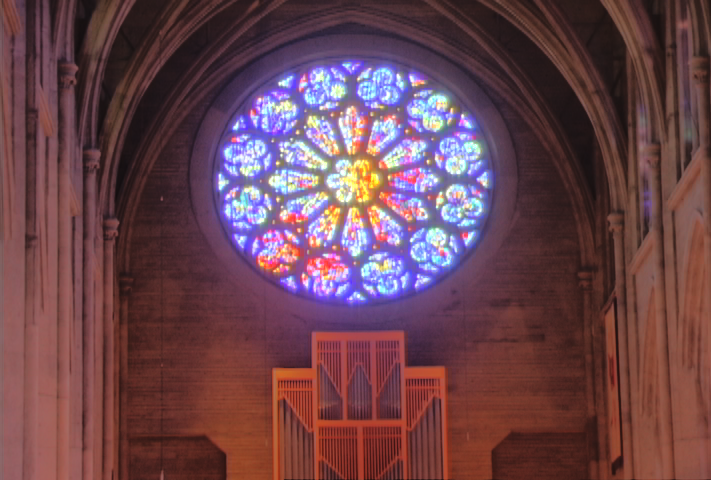
\includegraphics[scale=0.4]{rosette}
	\caption{Rosette scene mapped with our operator}
\end{figure}

\section{Performance}

We observe that the first step of the MMBEBHE algorithm is an $O(n^2)$ operation as each position's error requires a calculation relative to each luminance value. Chen et al. present a recursive divide-and-conquer strategy that reduces the problem to $O(n log n)$, however we have found that even with a 'brute force' approach computation time is sub-second using a modern processor (Intel Core 2 Duo) even on large images.

\section{Conclusion}

We have presented several enhancements to the original tone mapping technique that improve the output while simulatenously removing the need for extensive user input. By removing the need for the user to manually adjust the output we have made it possible for this tone mapping operator to be used on large volumes of high dynamic range content, making it suitable for processing image archives or high dynamic range video. Our addition of a local contrast enhancing step improves the image readability beyond what is possible with only global contrast enhancement. By adding these enhancements, we improve the output of this tone mapping operator while reducing demands on the user resulting in better and more consistent tone apped images.

\section{Acknowledgements}

We thank Paul Debevec, Rafal Mantiuk and all the authors who have made their HDR data publicly available. We also thank Igor Kravtchenko for making available his routines for loading RGBE (.HDR) images.

\pagebreak[4]
\bibliography{tonemappingbib}{}
\bibliographystyle{plain}

\end{document}